\documentclass[border=12pt]{standalone}
\usepackage{amsmath, amssymb}
\usepackage{tikz}
\definecolor{ring0}{HTML}{0033CC}
\definecolor{ring1}{HTML}{0066FF}
\definecolor{ring2}{HTML}{0099FF}
\definecolor{ring3}{HTML}{00CCCC}
\definecolor{ring4}{HTML}{00CC66}
\definecolor{ring5}{HTML}{33CC00}
\definecolor{ring6}{HTML}{99CC00}
\definecolor{ring7}{HTML}{CCCC00}
\definecolor{ring8}{HTML}{FF9900}
\definecolor{ring9}{HTML}{FF6600}
\definecolor{ring10}{HTML}{FF3300}
\definecolor{ring11}{HTML}{CC0000}
\definecolor{gap0}{HTML}{E53935}
\definecolor{gap1}{HTML}{1E88E5}
\definecolor{gapfar}{HTML}{CCCCCC}
\begin{document}
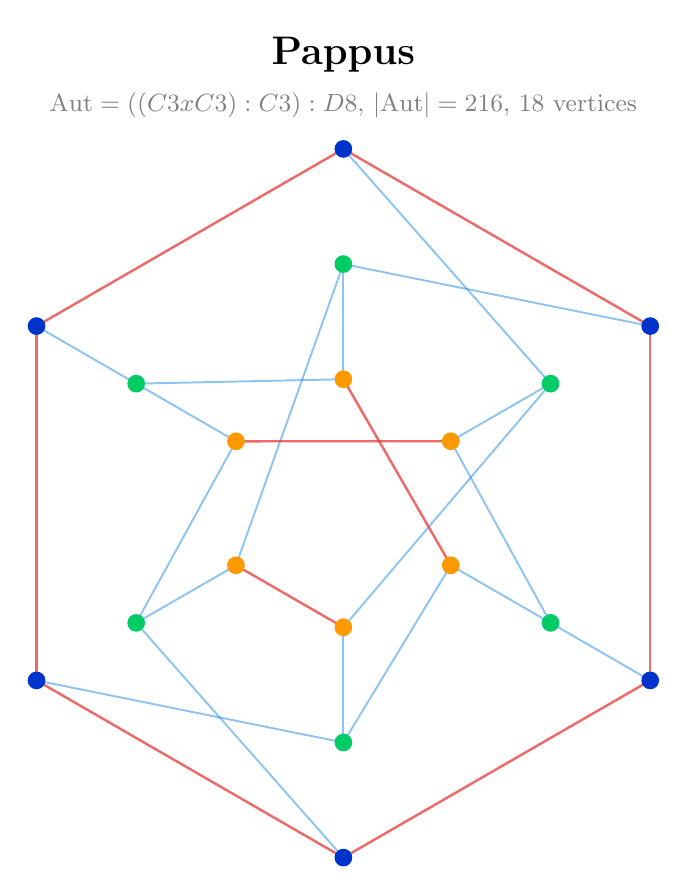
\begin{tikzpicture}
\node[font=\Large\bfseries] at (0, 5.70) {Pappus};
\node[font=\small, text=gray] at (0, 5.05) {$\mathrm{Aut} = ((C3 x C3) : C3) : D8$, $|\mathrm{Aut}| = 216$, 18 vertices};
\draw[line width=0.70pt, gap1, opacity=0.50] (0.000, 4.500) -- (2.631, 1.519);
\draw[line width=0.70pt, gap1, opacity=0.50] (-3.897, 2.250) -- (-2.631, 1.519);
\draw[line width=0.70pt, gap1, opacity=0.50] (-3.897, -2.250) -- (-0.000, -3.038);
\draw[line width=0.70pt, gap1, opacity=0.50] (-0.000, -4.500) -- (-2.631, -1.519);
\draw[line width=0.70pt, gap1, opacity=0.50] (3.897, -2.250) -- (2.631, -1.519);
\draw[line width=0.70pt, gap1, opacity=0.50] (3.897, 2.250) -- (0.000, 3.038);
\draw[line width=0.70pt, gap1, opacity=0.50] (0.000, 3.038) -- (0.000, 1.575);
\draw[line width=0.70pt, gap1, opacity=0.50] (0.000, 3.038) -- (-1.364, -0.788);
\draw[line width=0.70pt, gap1, opacity=0.50] (0.000, 1.575) -- (-2.631, 1.519);
\draw[line width=0.70pt, gap1, opacity=0.50] (-2.631, 1.519) -- (-1.364, 0.787);
\draw[line width=0.70pt, gap1, opacity=0.50] (-1.364, 0.787) -- (-2.631, -1.519);
\draw[line width=0.70pt, gap1, opacity=0.50] (-2.631, -1.519) -- (-1.364, -0.788);
\draw[line width=0.70pt, gap1, opacity=0.50] (-0.000, -1.575) -- (-0.000, -3.038);
\draw[line width=0.70pt, gap1, opacity=0.50] (-0.000, -1.575) -- (2.631, 1.519);
\draw[line width=0.70pt, gap1, opacity=0.50] (-0.000, -3.038) -- (1.364, -0.788);
\draw[line width=0.70pt, gap1, opacity=0.50] (1.364, -0.788) -- (2.631, -1.519);
\draw[line width=0.70pt, gap1, opacity=0.50] (2.631, -1.519) -- (1.364, 0.788);
\draw[line width=0.70pt, gap1, opacity=0.50] (1.364, 0.788) -- (2.631, 1.519);
\draw[line width=0.88pt, gap0, opacity=0.75] (0.000, 4.500) -- (-3.897, 2.250);
\draw[line width=0.88pt, gap0, opacity=0.75] (0.000, 4.500) -- (3.897, 2.250);
\draw[line width=0.88pt, gap0, opacity=0.75] (-3.897, 2.250) -- (-3.897, -2.250);
\draw[line width=0.88pt, gap0, opacity=0.75] (-3.897, -2.250) -- (-0.000, -4.500);
\draw[line width=0.88pt, gap0, opacity=0.75] (-0.000, -4.500) -- (3.897, -2.250);
\draw[line width=0.88pt, gap0, opacity=0.75] (3.897, -2.250) -- (3.897, 2.250);
\draw[line width=0.88pt, gap0, opacity=0.75] (0.000, 1.575) -- (1.364, -0.788);
\draw[line width=0.88pt, gap0, opacity=0.75] (-1.364, 0.787) -- (1.364, 0.788);
\draw[line width=0.88pt, gap0, opacity=0.75] (-1.364, -0.788) -- (-0.000, -1.575);
\fill[ring0] (0.000, 4.500) circle (3.2pt);
\fill[ring0] (-3.897, 2.250) circle (3.2pt);
\fill[ring0] (-3.897, -2.250) circle (3.2pt);
\fill[ring0] (-0.000, -4.500) circle (3.2pt);
\fill[ring0] (3.897, -2.250) circle (3.2pt);
\fill[ring0] (3.897, 2.250) circle (3.2pt);
\fill[ring4] (0.000, 3.038) circle (3.2pt);
\fill[ring8] (0.000, 1.575) circle (3.2pt);
\fill[ring4] (-2.631, 1.519) circle (3.2pt);
\fill[ring8] (-1.364, 0.787) circle (3.2pt);
\fill[ring4] (-2.631, -1.519) circle (3.2pt);
\fill[ring8] (-1.364, -0.788) circle (3.2pt);
\fill[ring8] (-0.000, -1.575) circle (3.2pt);
\fill[ring4] (-0.000, -3.038) circle (3.2pt);
\fill[ring8] (1.364, -0.788) circle (3.2pt);
\fill[ring4] (2.631, -1.519) circle (3.2pt);
\fill[ring8] (1.364, 0.788) circle (3.2pt);
\fill[ring4] (2.631, 1.519) circle (3.2pt);
\end{tikzpicture}
\end{document}